The previous chapter introduced the deterministic and stochastic sequential decision making problems, and demonstrated how these problems can be solved by dynamic programming. 
While dynamic programming is a powerful algorithm, it also suffers from several practical challenges. This chapter briefly introduces some of the key ideas in \textit{reinforcement learning}\cite{Bertsekas2019}\cite{SuttonBarto2018}, which encompasses a set of ideas that can generally be viewed as extensions or approximations of the dynamic programming approach, which make it more practical for many robotic applications.

\notessection{Reinforcement Learning}
Reinforcement learning (RL) is a broad field that studies autonomous decision making, including several more general and challenging problems than have been considered in previous chapters. 
In particular, the standard reinforcement learning problem is to determine closed-loop control policies that drive an agent to maximize an accumulated reward\footnote{Note that the maximization of ``reward'' in the context of reinforcement learning is essentially equivalent to minimization of ``cost'' in optimal control formulations}. However, in the most general case it is not required that a \textit{system model} be known! This paradigm can be represented by Figure \ref{fig:rl}, where it can be seen that given a control input the environment specifies the state and reward, and the environment can be considered to be a black box (it is not necessarily known how the state is generated).
\begin{figure}[ht]
    \centering
    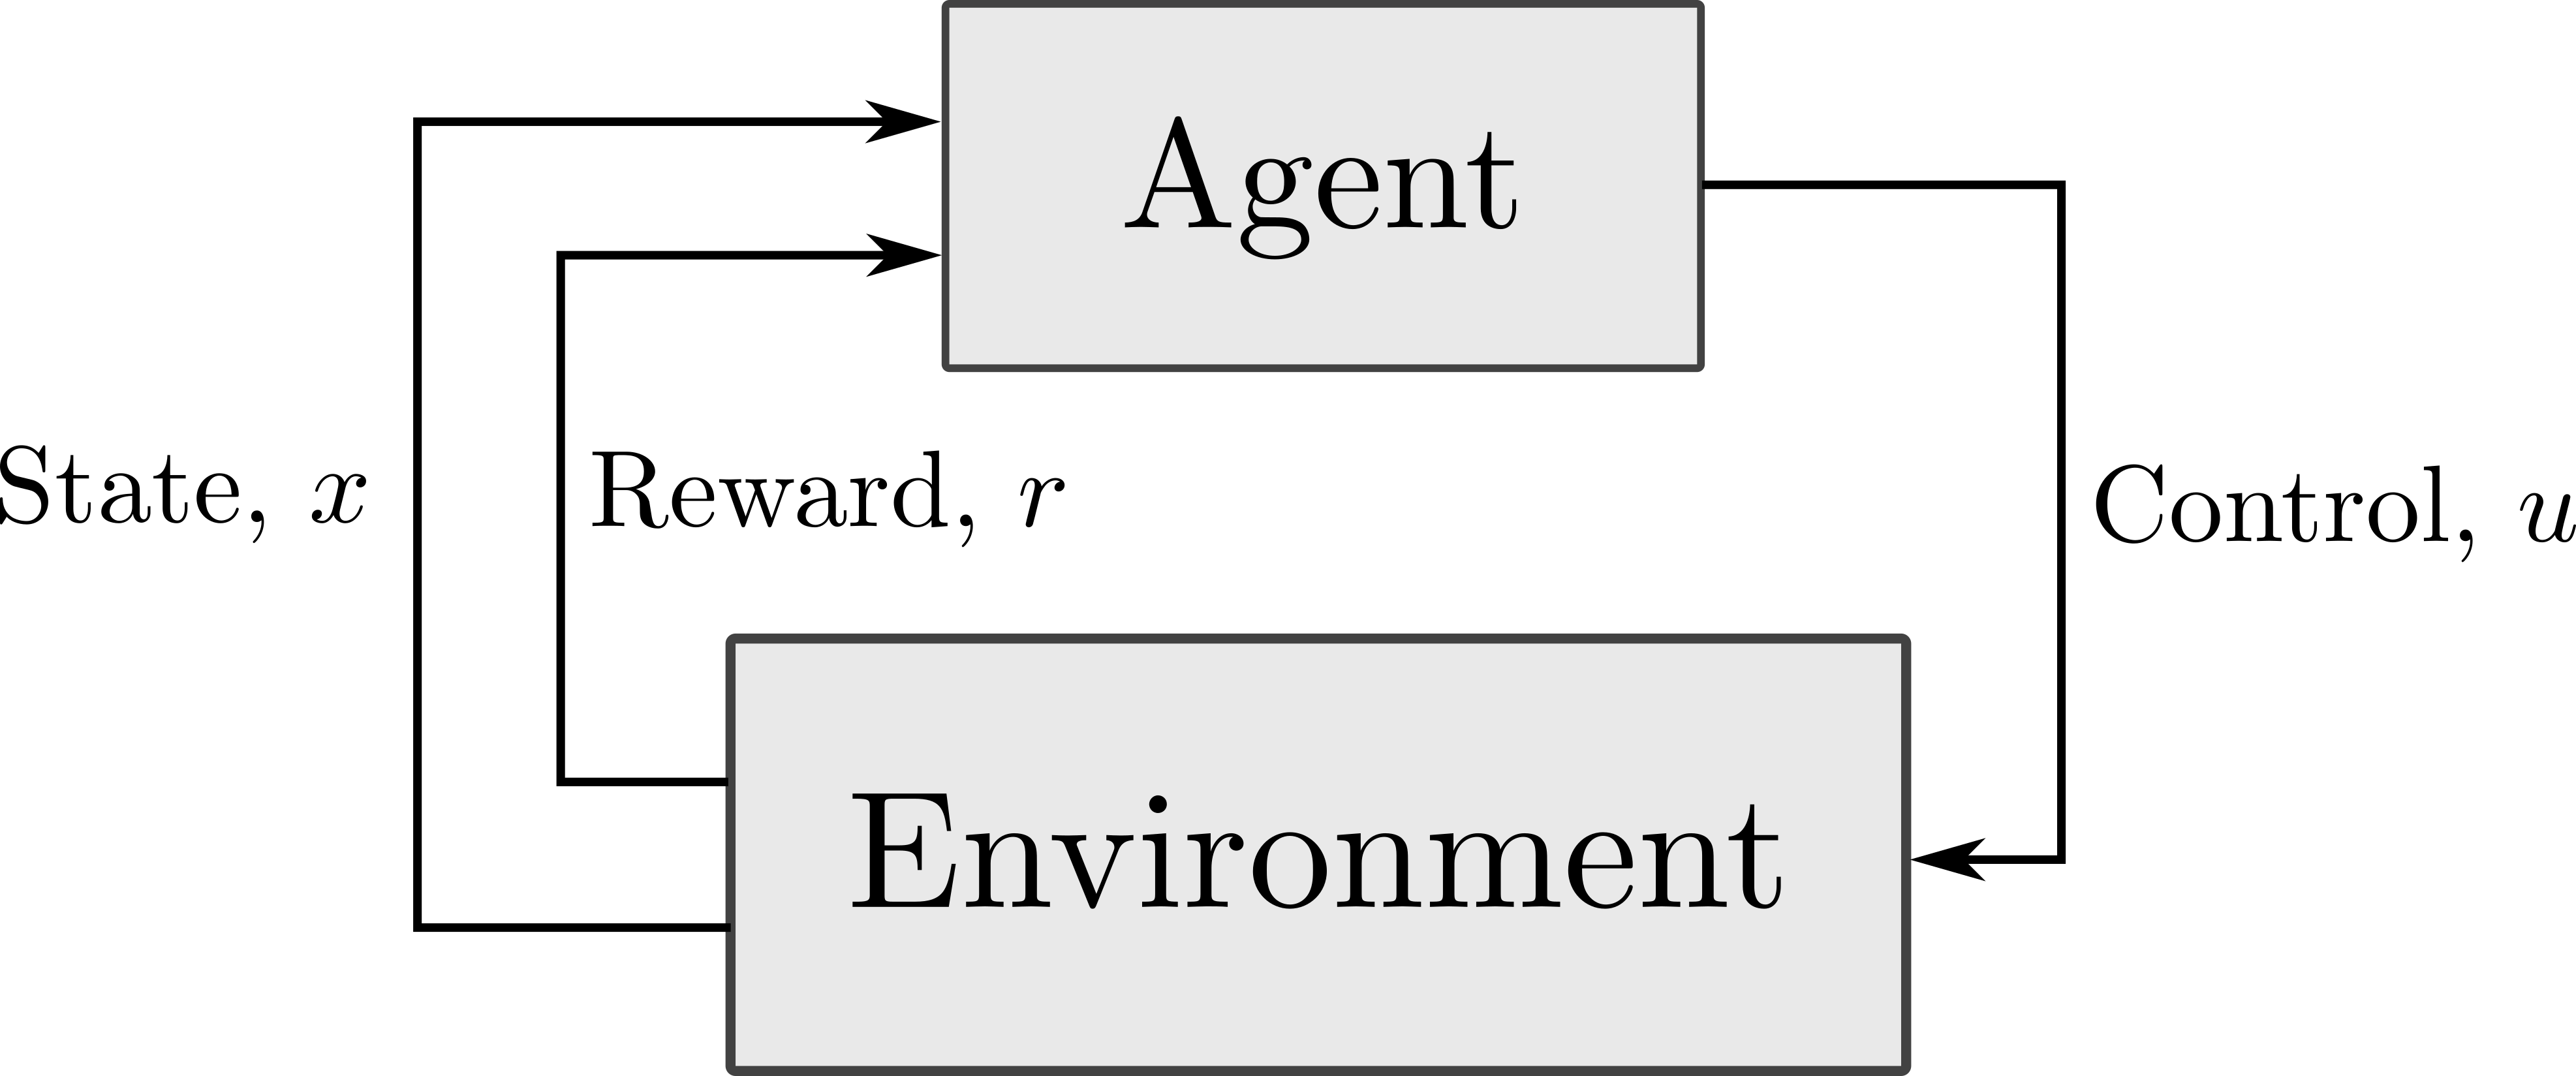
\includegraphics[width=0.6\textwidth]{tex/figs/ch21_figs/rl.png}
    \caption{In reinforcement learning problems, the robot (agent) learns how to make decisions by interacting with the environment.}
    \label{fig:rl}
\end{figure}

Reinforcement learning is a highly active field of research, and has seen successes in several applications including acrobatic control of helicopters, games, finance, and robotics. In this chapter the fundamentals of reinforcement learning are introduced, including the formulation of the RL problem, RL algorithms that leverage system models (value iteration/dynamic programming and policy iteration), and a few RL algorithms that do not require system models (Q-learning, policy gradient, actor-critic). 

\subsection{Problem Formulation}
The reinforcement learning problem is effectively the same as the stochastic decision making problem from the previous chapter, but a slightly different notation will be used\footnote{The fields of optimal control and reinforcement learning have significant overlap, but each community has developed its own standard notation. Most often, the state in the optimal control community is represented by $\x$ and in the RL community as $\bm{s}$. Similarly, in control theory the control input is $\bu$ while in the RL community it is referred to as an action $\bm{a}$.}. The state and control input for the system is denoted as $\x$ and $\bu$, and the set of admissible states and controls are denoted as $\mathcal{X}$ and $\mathcal{U}$. However, the stochastic state transition model will now be written as:
\begin{equation} \label{eq:RLmodel}
p(\x_t \mid \x_{t-1}, \bu_{t-1}),
\end{equation}
which is the conditional probability distribution over $\x_t$, given the previous state and control. 

As was the case for the stochastic decision making problem from previous chapter, RL algorithms seek to compute \textit{policies} $\pi = \{\pi_0, \pi_1, \dots, \pi_{T-1}\}$ that define the control:
\begin{equation} \label{eq:RLpolicy}
\bu_t = \pi_t(\x_t),
\end{equation}
which results in a closed-loop control law.
However, instead of a ``cost'' function (that was used in the previous chapter), reinforcement learning problems are typically formulated with a \textit{reward} function:
\begin{equation} \label{eq:RLreward}
r_t = R(\x_t, \bu_t),
\end{equation}
where $r_t$ is the reward for being at state $\x_t$ and applying a control $\bu_t$. The goal of the reinforcement learning problem is to maximize the accumulated reward over a number of time steps (in contrast to minimizing cost in the previous chapter). Specifically, the total expected (discounted) reward over $T$ time steps is defined for a particular policy $\pi$ as:
\begin{equation} \label{eq:RLvalue}
V_T^\pi(\x) = E\big[\sum_{t=0}^{T-1} \gamma^tR(\x_t, \pi_t(\x_t)) \mid \x_0 = \x \big],
\end{equation}
where $\gamma \in (0,1]$ is referred to as a \textit{discount factor}, and the function $V_T^\pi(\x)$ is referred to as the \textit{value function}\footnote{Notice the similarity of the value function to the expected cost in the stochastic decision making problem from the previous chapter.} for the policy $\pi$ (starting from $\x$ and with $T$ steps to go). The discount factor $\gamma$ was not used in the decision making problems from the previous chapter, and can be chosen as $\gamma = 1$ for finite horizon problems. However, it is common in RL problems to consider infinite horizons $T = \infty$, and in this case the discount factor must be chosen such that $\gamma < 1$ to ensure the expected reward is finite\footnote{The term ``discount factor'' is used because it ``discounts'' future rewards. The intuition behind this can be explained by the phrase ``a dollar today is better than a dollar tomorrow''.}. 

The reinforcement learning problem is therefore to find a optimal policy $\pi^*$ that maximizes the expected reward (i.e. maximizes the value function):
\begin{definition}[Reinforcement Learning Problem]
The reinforcement learning problem for the system model \eqref{eq:RLmodel}, admissible states $\x \in \mathcal{X}$ and controls $\bu \in \mathcal{U}$, and reward function \eqref{eq:RLreward} is to find an optimal policy $\pi^*$ that satisfies:
\begin{equation} \label{eq:rlproblem}
\pi^*(\x) = \underset{\pi}{\arg\max} \:\: V_T^\pi(\x),
\end{equation}
for all states $\x \in \mathcal{X}$.
\end{definition}


\subsection{Model-based Reinforcement Learning}
Model-based reinforcement learning methods rely on the use of an explicit parameterization of the transition model \eqref{eq:RLmodel}. While this model could come from physics-based modeling techniques, in many RL settings the model might also be learned from data! For example, for discrete state/action spaces it is possible to empirically approximate the transition probabilities $p(\x_t \mid \x_{t-1}, \bu_{t-1})$ for every pair $(\x_t,\bu_t)$ by counting the number of times each transition occurs in the dataset! More sophisticated models include linear models generated through least squares, or Gaussian process or neural network models trained through an appropriate loss function.

\subsubsection{Value Iteration (Dynamic Programming)}
While the dynamic programming algorithm was covered in the previous chapter, it will also be included here in the context of the reinforcement learning problem formulation. In this case, the ``principle of optimality'' again says that the optimal \textit{tail} policy is optimal for \textit{tail} subproblems, which leads to the recursion:
\begin{equation} \label{eq:RLbellman}
V^*_{k+1}(\x) = \underset{\bu \in \mathcal{U}}{\max} \:\:R(\x, \bu) + \gamma \sum_{\x'} p(\x' \mid \x, \bu) V^*_{k}(\x'),
\end{equation}
which is commonly referred to as the \textit{Bellman equation} (note that a shorthand $V^*_{k}(\x) = V^{\pi^*}_{k}(\x)$ is used for the optimal value function). In words, this expression says that the optimal reward associated with starting at the state $\x$ and having $k+1$ steps to go can be found as an optimization over the immediate control by accounting for the (expected) optimal tail rewards.
The full dynamic programming algorithm for solving the RL problem \eqref{eq:rlproblem} is given in Algorithm \ref{alg:RLdp}.
\begin{algorithm}[ht]
 $V_0^*(\x) = 0,$ for all $\x \in \mathcal{X}$\\
 \For{$k=0$ \KwTo $T-1$}{
  $V_{k+1}^*(\x) = \underset{\bu \in \mathcal{U}}{\max} \:\:R(\x, \bu) + \gamma \sum_{\x'} p(\x' \mid \x, \bu) V^*_{k}(\x'),$ for all $\x \in \mathcal{X}$\\
  $\pi_{T-1-k}^*(\x) = \underset{\bu \in \mathcal{U}}{\arg \max} \:\:R(\x, \bu) + \gamma \sum_{\x'} p(\x' \mid \x, \bu) V^*_{k}(\x'),$ for all $\x \in \mathcal{X}$\\
 }
 \Return $V^*_0(\cdot),\dots,V^*_T(\cdot), \pi^*_0(\cdot),\dots,\pi^*_{T-1}(\cdot)$
 \caption{Dynamic Programming (Reinforcement Learning)}
 \label{alg:RLdp}
\end{algorithm}

In the context of reinforcement learning, this procedure is commonly referred to as \textit{value iteration} and in many cases it is assumed that the horizon $T$ is infinite. For infinite-horizon problems the ``value iteration'' in Algorithm \ref{alg:RLdp} is performed either over a finite-horizon (which yields an approximate solution), or until convergence to a stationary (i.e. time-invariant) optimal value function/policy\footnote{In the infinite horizon case, the optimal value function is unique and the optimal policy is stationary and deterministic, but not necessarily unique.}.

To solidify the relationship between value iteration in the context of RL and dynamic programming in the context of stochastic decision making from the previous chapter, the inventory control example from the previous chapter is revisited:
\begin{example}[Inventory Control] \label{ex:RLDP}
\theoremstyle{definition}
Consider again the inventory control problem from the previous chapter, where the available stock of a particular item is the state $x_t \in \mathbb{N}$, the control $u_t \in \mathbb{N}$ adds items to the inventory, the demand $w_t$ is uncertain, and the dynamics and constraints are:
\begin{equation*}
\begin{split}
&x_{t} = \max \{0, x_{t-1} + u_{t-1} - w_{t-1}\}, \\
&p(w=0) = 0.1, \quad p(w = 1) = 0.7, \quad p(w = 2) = 0.2.
\end{split}
\end{equation*}
and
\begin{equation*}
x_t + u_t \leq 2.
\end{equation*}
Based on the dynamics, the probabilistic model \eqref{eq:RLmodel} is given by:
\begin{equation*}
\begin{split}
p(x_{t} = \{0, 1, 2\} \mid x_{t-1} = 0, u_{t-1} = 0) &= \{1, 0, 0\}, \\
p(x_{t} = \{0, 1, 2\} \mid x_{t-1} = 0, u_{t-1} = 1) &= \{0.9, 0.1, 0\}, \\
p(x_{t} = \{0, 1, 2\} \mid x_{t-1} = 0, u_{t-1} = 2) &= \{0.2, 0.7, 0.1\}, \\
p(x_{t} = \{0, 1, 2\} \mid x_{t-1} = 1, u_{t-1} = 0) &= \{0.9, 0.1, 0\}, \\
p(x_{t} = \{0, 1, 2\} \mid x_{t-1} = 1, u_{t-1} = 1) &= \{0.2, 0.7, 0.1\}, \\
p(x_{t} = \{0, 1, 2\} \mid x_{t-1} = 2, u_{t-1} = 0) &= \{0.2, 0.7, 0.1\}, \\
\end{split}
\end{equation*}
where some transition values are not explicitly written due to the control constraints.
Next, the reward function is defined as:
\begin{equation*}
\begin{split}
R(x_t,u_t) &= -E\big[u_t + (x_t + u_t - w_t)^2\big] , \\
&= -\big(u_t + (x_t + u_t - E[w_t])^2 + Var(w_t)\big), \\
\end{split}
\end{equation*}
and a discount factor of $\gamma=1$ is used. As in the previous chapter, this reward penalizes (a negative reward is a penalty) ordering new stock and having available stock at the next time step (i.e. having to store stock).

Algorithm \ref{alg:RLdp} can now be applied, starting with the value function with no steps to go:
\begin{equation*}
V^*_0(x) = 0,
\end{equation*}
and then recursively computing:
\begin{equation*}
\begin{split}
V^*_1(0) &= \underset{u \in \{0,1,2\}}{\max} -\big(u + (u - 1.1)^2 + 0.29\big) = -1.3, \\
V^*_1(1) &= \underset{u_2 \in \{0,1\}}{\max} -\big(u + (1 + u - 1.1)^2 + 0.29\big) = -0.3,\\
V^*_1(2) &= -\big((2 - 1.1)^2 + 0.29\big) = -1.1, \\
\end{split}
\end{equation*}
where $E[w] = 1.1$ and $Var(w) = 0.29$.
The optimal stage policies associated with this step are:
\begin{equation*}
\begin{split}
\pi^*_{T-1}(0) = 1, \quad \pi^*_{T-1}(1) = 0, \quad \pi^*_{T-1}(2) = 0.
\end{split}
\end{equation*}
In the next step:
\begin{equation*}
\begin{split}
V^*_2(0) &= \underset{u \in \{0,1,2\}}{\max} -\big(u + (u - 1.1)^2 + 0.29\big) + \sum_{x'} p(x' \mid x=0, u)V^*_1(x') = -2.5, \\
V^*_2(1) &= \underset{u \in \{0,1,\}}{\max} -\big(u + (1 + u - 1.1)^2 + 0.29\big) + \sum_{x'} p(x' \mid x=1, u)V^*_1(x') = -1.5,\\
V^*_2(2) &= -\big((2 - 1.1)^2 + 0.29\big) + \sum_{x'} p(x' \mid x=2, u=0)V^*_1(x') = -1.68,\\
\end{split}
\end{equation*}
with optimal stage policies:
\begin{equation*}
\begin{split}
\pi^*_{T-2}(0) = 1, \quad \pi^*_{T-2}(1) = 0, \quad \pi^*_{T-2}(2) = 0.
\end{split}
\end{equation*}
Finally, in the last step:
\begin{equation*}
\begin{split}
V^*_3(0) &= \underset{u \in \{0,1,2\}}{\max} -\big(u + (u - 1.1)^2 + 0.29\big) + \sum_{x'} p(x' \mid x=0, u)V^*_2(x') = -3.7, \\
V^*_3(1) &= \underset{u \in \{0,1,\}}{\max} -\big(u + (1 + u - 1.1)^2 + 0.29\big)  + \sum_{x'} p(x' \mid x=1, u)V^*_2(x')= -2.7,\\
V^*_3(2) &= -\big((2 - 1.1)^2 + 0.29\big)  + \sum_{x'} p(x' \mid x=2, u=0)V^*_2(x') = -2.818,\\
\end{split}
\end{equation*}
with optimal stage policies:
\begin{equation*}
\begin{split}
\pi^*_{T-3}(0) = 1, \quad \pi^*_{T-3}(1) = 0, \quad \pi^*_{T-3}(2) = 0. 
\end{split}
\end{equation*}
These results are, in fact, identical to the results from the example in the previous chapter! The only difference is the formulation of the problem in the RL framework instead of the stochastic decision making problem framework.
\end{example}


\subsubsection{Policy Iteration}
Another common algorithm that can be used to solve the reinforcement learning problem \eqref{eq:rlproblem} is \textit{policy iteration}. The main idea of policy iteration is that if the value function can be computed for any arbitrary policy $\pi=\{\pi_0, \pi_1, \dots, \pi_{T-1}\}$, then the policy can be incrementally improved to yield a better policy $\pi'=\{\pi_0', \pi_1', \dots, \pi_{T-1}'\}$.

\paragraph{Policy Evaluation:}
The first key element of the policy iteration algorithm is \textit{policy evaluation}, which is used to compute the value function $V_k^\pi(\x)$ for a given policy $\pi$. Policy evaluation is based on the recursion:
\begin{equation} \label{eq:RLpolicyeval}
V^\pi_{k+1}(\x) = R(\x, \pi(\x)) + \gamma \sum_{\x'} p(\x' \mid \x, \pi(\x)) V^*_{k}(\x'),
\end{equation}
which is very similar to the Bellman equation \eqref{eq:RLbellman} except that there is no optimization over the control (since it is fixed). The policy evaluation algorithm is given in Algorithm \ref{alg:RLpolicyeval}.
\begin{algorithm}[ht]
 \KwData{$\pi$}
 \KwResult{$V^\pi_0(\cdot),\dots,V^\pi_T(\cdot)$}
 $V_0^\pi(\x) = 0,$ for all $\x \in \mathcal{X}$\\
 \For{$k=0$ \KwTo $T-1$}{
  $V_{k+1}^\pi(\x) = R(\x, \pi_{T-1-k}(\x)) + \gamma \sum_{\x'} p(\x' \mid \x, \pi_{T-1-k}(\x)) V^\pi_{k}(\x'),$ for all $\x \in \mathcal{X}$\\
 }
 \Return $V^\pi_0(\cdot),\dots,V^\pi_T(\cdot)$
 \caption{Policy Evaluation}
 \label{alg:RLpolicyeval}
\end{algorithm}

In the infinite-horizon case where a stationary policy is used, the iteration in Algorithm \ref{alg:RLpolicyeval} stops when the value function has converged to its stationary value. 
Indeed, since the infinite horizon value function is the stationary point of this recursion, it is possible to directly solve for it by setting both $V^\pi_{k+1} = V^\pi_{k} = V^\pi_\infty$ in \eqref{eq:RLpolicyeval}. In the case of a discrete state space with $N$ possible states, this creates a linear system of $N$ equations which can be used to solve for $V^\pi_\infty$ directly.

\paragraph{Q-function:}
The second key component in the policy iteration algorithm is the state-action value function, which is also referred to as the \textit{Q-function}. Unlike the value function, the Q-function is a function of both state and control:
\begin{equation} \label{eq:RLqfunc}
Q^\pi_{k+1}(\x,\bu) = R(\x, \bu) + \gamma \sum_{\x'} p(\x' \mid \x, \bu) V^\pi_{k}(\x'),
\end{equation}
and can be interpreted as the ``value'' of starting in state $\x$, applying control $\bu$, and then following the policy $\pi$ for the remaining time. In other words, it specifies the value associated with deviating from the given policy $\pi$ for a single time-step.

Similarly, the \textit{optimal} Q-function is:
\begin{equation*}
Q^*_{k+1}(\x,\bu) = R(\x, \bu) + \gamma \sum_{\x'} p(\x' \mid \x, \bu) V^*_{k}(\x'),
\end{equation*}
where the shorthand notation $Q^*_{k}(\x,\bu) = Q^{\pi^*}_{k}(\x,\bu)$ is used.
Note that from the Bellman equation \eqref{eq:RLbellman} the optimal value function can be written as an optimization over the optimal Q-function:
\begin{equation*}
V^*_{k+1}(\x) = \underset{\bu \in \mathcal{U}}{\max} \:\: Q^*_{k+1}(\x,\bu).
\end{equation*}
Therefore, instead of computing the optimal value function using value iteration it is possible to deal directly with the Q-function!

\paragraph{Policy Iteration Algorithm:}
The policy iteration algorithm incrementally updates the policy by performing local optimizations of the Q-function. In particular, a single iteration of the policy update is shown in Algorithm \ref{alg:RLpolicyiter}.
\begin{algorithm}[ht]
 \KwData{$\pi$}
 \KwResult{$\pi'$}
 $V^\pi_0(\cdot),\dots,V^\pi_T(\cdot) \xleftarrow{}$ PolicyEvaluation($\pi$)\\
 \For{$k=0$ \KwTo $T-1$}{
  $Q^\pi_{k+1}(\x,\bu) = R(\x, \bu) + \gamma \sum_{\x'} p(\x' \mid \x, \bu) V^\pi_{k}(\x')$ for all $\x \in \mathcal{X}$\\
  $\pi'_{T-1-k}(\x) = \underset{\bu \in \mathcal{U}}{\arg \max} \:\:Q^\pi_{k+1}(\x,\bu),$ for all $\x \in \mathcal{X}$\\
 }
 \Return $\pi' = \{\pi'_0, \dots, \pi'_{T-1} \}$
 \caption{Policy Iteration Step}
 \label{alg:RLpolicyiter}
\end{algorithm}
It can be proven theoretically that under the policy iteration algorithm the value function is monotonically increasing with each new policy, and the procedure is run until convergence.
While policy iteration and value iteration are quite similar, policy iteration can end up converging faster in some cases.

\subsection{Model-free Reinforcement Learning}
The value and policy iteration algorithms are applicable only to problems where the probabilistic system model $p(\x_t \mid \x_{t-1}, \bu_{t-1})$ is \textit{known}. In many real-world robotics applications this may not be the case!

In general, many reinforcement learning algorithms address problems where it is assumed that the agent only has access to the rewards $r_t$ and states $\x_t$, but does not know how they are generated. Therefore the agent must ``learn'' policies from experience, or in other words from trajectory data:
\begin{equation*}
\{\x_0, \x_1, \dots, \x_T \}, \quad \{\bu_0, \bu_1, \dots, \bu_{T-1} \}, \quad \{r_0, r_1, \dots, r_{T-1} \}.
\end{equation*}

\subsubsection{Q-Learning}
One algorithm for solving the more challenging model-free problem is \textit{Q-learning}. 
The core idea behind Q-learning is that it is possible to collect data samples $(\x_t, \bu_t, r_t, \x_{t+1})$, and over time learn what the optimal Q-function $Q^*(\x, \bu)$ is.
For simplicity an infinite-horizon ($T=\infty$) problem will be considered, such that the optimal value and Q-functions will be stationary, and in particular the optimal Q-function will satisfy:
\begin{equation*}
Q^*(\x,\bu) = R(\x, \bu) + \gamma \sum_{\x'} p(\x' \mid \x, \bu) \max_{\bu'\in \mathcal{U}} Q^*(\x', \bu').
\end{equation*}

Importantly, even if the model and reward function are unknown, for a given sample $(\x_t, \bu_t, r_t, \x_{t+1})$ that is collected by interacting with the environment, the \textit{expectation}:
\begin{equation*}
E\big[\big(r_t + \gamma \max_{\bu'\in \mathcal{U}} Q^*(\x_{t+1}, \bu')\big) - Q^*(\x_t,\bu_t)\big] = 0,
\end{equation*}
will hold for the optimal Q-function. Therefore, the idea of Q-learning is that an approximation of the optimal Q-function can be improved over time by collecting data and trying to ensure that the above conditions holds. This leads to the Q-learning algorithm described in Algorithm \ref{alg:Q-learning}.

\begin{algorithm}[ht]
 \KwData{Set $\mathcal{S}$ of trajectory samples $\{\x_t, \bu_t, r_t, \x_{t+1}\}$, learning rate $\alpha$}
 \KwResult{$Q(\x, \bu)$}
 Initialize $Q(\x, \bu) $ for all $\x \in \mathcal{X}$ and $\bu \in \mathcal{U}$\\
 \For{$\{\x_t, \bu_t, r_t, \x_{t+1}\} \in \mathcal{S}$}{
  $Q(\x_t,\bu_t) \xleftarrow{} Q(\x_t,\bu_t) + \alpha\Big(r_t + \gamma \max_{\bu \in \mathcal{U}} Q(\x_{t+1}, \bu) - Q(\x_t,\bu_t)  \Big) $\\
 }
 \Return $Q(\x, \bu)$
 \caption{Q-learning}
 \label{alg:Q-learning}
\end{algorithm}

Q-learning is referred to as a \textit{model-free} method because it 
forgoes explicitly estimating the true (unknown) system dynamics, and directly estimates the Q-function.
It is also called a \textit{value-based} model-free method since it does not directly build the policy, but rather estimates the optimal Q-function to implicitly define the policy.

Q-learning can be guaranteed to converge to the optimal Q-function under certain conditions, but has some practical disadvantages. In particular, unless the number of possible states and controls are finite and relatively small, it can be intractable to store the Q-value associated with each state-value pair. One variation of the Q-learning algorithm to handle large or continuous state  and control spaces is to parameterize the Q-function as $Q_{\btheta}(\x, \bu)$ and to simply update the parameters $\theta$. While this method often works well in practice, convergence is not guaranteed. Another disadvantage of Q-learning is that sometimes the Q-function can be complex and therefore potentially hard to learn.

\subsubsection{Policy Gradient}
The \textit{policy gradient} method for reinforcement learning problems can also be applied to situations where the model is unknown. This approach, which directly optimizes the policy, can be particularly useful for scenarios where the optimal policy may be relatively simple compared to the Q-function, in which case Q-learning may be challenging. 

In the policy gradient approach, a class of \textit{stochastic}\footnote{A stochastic policy defines a distribution over actions at a given state, is useful for exploration, and sometimes is even required for optimality.} candidate policies $\pi_{\btheta}(\bu_t \mid \x_t)$ is defined based on a set of parameters $\btheta$, and the goal is to \textit{directly} modify the parameters $\btheta$ to improve performance. This is accomplished by using trajectory data to estimate a gradient of the performance with respect to the policy parameters $\btheta$, and then using the gradient to update $\btheta$. Because this method works directly on a policy (and does not learn a model or value function), it is referred to as a \textit{model-free} \textit{policy-based} approach.

Considering the original problem \eqref{eq:rlproblem}, the objective function can be written as:
\begin{equation*}
    J(\btheta) = E\big[\sum_{t=0}^{T-1} \gamma^tR(\x_t, \pi_{\btheta}(\bu_t \mid \x_t))\big],
\end{equation*}
where the $J(\btheta)$ notation is used to explicitly show the dependence on the parameters. Implementing a policy gradient approach therefore requires the computation of $\nabla_{\btheta} J(\btheta)$. One of the most common approaches is to \textit{estimate} this quantity using data, using what is known as a \textit{likelihood ratio method}.

Let $\tau$ represent a \textit{trajectory} of the system (consisting of sequential states and actions) under the current policy $\pi_{\btheta}(\bu_t \mid \x_t)$. As a shorthand notation, consider the total discounted reward over a trajectory $\tau$ to be defined written as:
\begin{equation} \label{eq:trajreward}
    r(\tau) = \sum_{t=0}^{T-1} \gamma^tR(\x_t, \pi_{\btheta}(\bu_t \mid \x_t),
\end{equation}
such that $J(\btheta)$ can be expressed equivalently as $J(\btheta) = E\big[r(\tau)\big]$. Additionally, let the probability that the trajectory $\tau$ occurs be expressed by the distribution $p_{\btheta}(\tau)$. Then the expectation from the objective function can be expanded as:
\begin{equation*}
J(\btheta) = \int_\tau r(\tau)p_{\btheta}(\tau) d\tau,
\end{equation*}
and its gradient given by\marginnote{From standard calculus $\nabla_{\btheta} \log p_{\btheta}(\tau) = \frac{1}{p_{\btheta}(\tau)} \nabla_{\btheta} p_{\btheta}(\tau)$, which replaces the use of the gradient $\nabla_{\btheta} p_{\btheta}(\tau)$ with $\nabla_{\btheta} \log p_{\btheta}(\tau)$. This is a very useful ``trick'' when it comes to approximately computing the integral, as will be seen shortly.}:
\begin{equation*}
\nabla_{\btheta} J(\btheta) = \int_\tau r(\tau)p_{\btheta}(\tau) \nabla_{\btheta} \log p_{\btheta}(\tau) d\tau.
\end{equation*}
Rather than explicitly computing this integral it is much easier to approximate using sampled data (i.e. sampled trajectories). This is possible since the integral can be written as the expectation $\nabla_{\btheta} J(\btheta) = E\big[r(\tau)\nabla_{\btheta} \log p_{\btheta}(\tau)\big]$, which can be estimated using a Monte Carlo method. While in general a number of sampled trajectories could be used to estimate the gradient, for data efficiency it is also possible to just use a single sampled trajectory $\tau$ and approximate:
\begin{equation} \label{eq:policygradapprox}
\nabla_{\btheta} J(\btheta) \approx r(\tau) \nabla_{\btheta} \log p_{\btheta}(\tau).
\end{equation}
In particular the sampled quantities $r(\tau)$ can be directly computed from \eqref{eq:trajreward}, and it turns out that the term $\nabla_{\btheta} \log p_{\btheta}(\tau)$ can be evaluated quite easily as\footnote{Using Bayes' rule: $p_{\btheta}(\tau) = p(\x_0) \Pi_{t=1}^{T-1} p(\x_t \mid \x_{t-1}, \bu_{t-1})\pi_{\btheta}(\x_{t-1} \mid \bu_{t-1})$. Then the $\log$ converts the product into a sum.}:
\begin{equation} \label{eq:gradlogterm}
\nabla_{\btheta} \log p_{\btheta}(\tau) = \sum_{t=0}^{T-1} \nabla_{\btheta} \log \pi_{\btheta}(\bu_t \mid \x_t).
\end{equation}
Importantly, notice that only the gradient of the policy is needed, and knowledge of the transition model $p(\x_t \mid \x_{t-1}, \bu_{t-1})$ is not! This occurs because only the policy is dependent on the parameters $\btheta$.

In summary, the gradient of $J(\theta)$ can be approximated given a trajectories $\tau$ under the current policy $\pi_{\btheta}$ by:
\begin{enumerate}
\item Compute $r(\tau)$ for the sampled trajectory using \eqref{eq:trajreward}.
\item Compute $\nabla_{\btheta} \log p_{\btheta}(\tau)$ for the sampled trajectory using \eqref{eq:gradlogterm}, which only requires computing gradients related to the current policy $\pi_{\btheta}$.
\item Approximate $\nabla_{\btheta} J(\btheta)$ using \eqref{eq:policygradapprox}.
\end{enumerate}
The process of sampling trajectories from the current policy, approximating the gradient, and performing a gradient descent step on the parameters $\btheta$ is referred to as the \textit{REINFORCE} algorithm\footnote{There are some other modified versions of this algorithm, for example some contain a baseline term $b(\x_0)$ in the gradient by replacing $r(\tau)$ with $r(\tau) - b(\x_0)$ to reduce the variance of the Monte Carlo estimate.}.

In general, policy-based RL methods such as policy gradient can converge more easily than value-based methods, can be effective in high-dimensional or continuous action spaces, and can learn stochastic policies. However, one challenge with directly learning policies is that they can get trapped in undesirable local optima. Policy gradient methods can also be data inefficient since they require data from the \textit{current} policy for each gradient step and cannot easily reuse old data.
This is in contrast to Q-learning, which is agnostic to the policy used and therefore doesn't waste data collected from past interactions.

\subsubsection{Actor-Critic}
Another popular reinforcement learning algorithm is the \textit{actor-critic} algorithm, which blends the concepts of value-based and policy-based model-free RL. In particular, a parameterized policy $\pi_{\btheta}$ (actor) is learned through a policy gradient method along side an estimated value function for the policy (critic). The addition of the critic helps to reduce the variance in the gradient estimates for the actor policy, which makes the overall learning process more data-efficient\footnote{This is a similar variance reduction approach to adding a baseline $b(\x_\tau)$ to the REINFORCE. In fact the baseline is chosen as the value function!}.

In particular, the policy $\pi_{\btheta}$ is again learned through policy gradient like in the REINFORCE algorithm, but with the addition of a learned approximation of the value function $V_{\bphi}(\x)$ as a baseline:
\begin{equation*}
\nabla_{\btheta} J(\btheta) \approx \sum_{t=0}^{T-1}  \big(r(\tau) - V_{\bphi}(\x_0)\big) \nabla_{\btheta} \log \pi_{\btheta}(\bu_t \mid \x_t).
\end{equation*}
Recall that the value function $V(\x)$ quantifies the expected total return starting from state $\x$ (i.e. the average performance). Therefore the quantity $r(\tau) - V_{\bphi}(\x_0)$ now represents a performance increase over average. Of course in this method the learned value function approximation $V_{\bphi}(\x)$ is also updated along with the policy by performing a similar gradient descent on the parameters $\bphi$.

\subsection{Deep Reinforcement Learning}
Neural networks are a powerful function approximator that can be utilized in reinforcement learning algorithms. For example, in Q-learning the Q-function can be approximated by a neural network to extend the approach to nonlinear, continuous state space domains. In policy gradient methods, the policy $\pi_{\btheta}$ can be parameterized as a neural network, enabling the policy to operate on high-dimensional states including images (i.e. visual feedback)!

\subsection{Exploration vs Exploitation}
When learning from experience (e.g. using Q-learning, policy gradient, actor-critic, deep RL, etc.) it is important to ensure that the experienced trajectories (i.e. the collected data points) are meaningful! For example, an abundance of data related to a particular set of actions/states will not necessarily be sufficient to learn good policies for \textit{all} possible situations. Therefore an important part of reinforcement learning is \textit{exploring} different combinations of states and actions. One simple approach to exploration is referred to as $\epsilon$-greedy exploration, where a random control is applied instead of the current (best) policy with probability $\epsilon$. 

However, exploration can lead to suboptimal performance since any knowledge accumulated about the optimal policy is ignored\footnote{In other words, actions with known rewards may be foregone in the hope that exploring leads to an even better reward.}. This leads to the \textit{exploration vs exploitation} trade-off: a fundamental challenge in reinforcement learning.